\documentclass[UTF8,a4paper]{paper}
\usepackage{ctex}
\usepackage[utf8]{inputenc}
\usepackage{amsmath}
\usepackage{amssymb}
\usepackage{pdfpages}
\usepackage{graphicx}
\usepackage{xcolor}
\title{模式识别作业7}
\author{张蔚桐\ 2015011493\ 自55}
\begin {document}
\maketitle
\section{}
\subsection{}
首先我们定义如下表达式来简化表述
\begin{equation}
\epsilon(i,j)\triangleq\epsilon_i(x_j)\triangleq h_i(x_j)-y(x_j)
\label{1}
\end{equation}
为表述所有分类器对所有样本预测的偏差。

于是对于$m$个单独的分类器,他们的平均均方误差可以定义为
\begin{equation}
E_h=\frac{1}{m}\sum_{i=i}^m[\frac{1}{n}\sum_{j=1}^n(\epsilon(i,j)^2)]
\label{2}
\end{equation}
\begin{equation}
E_{h_B}=\frac{1}{n}\sum_{j=1}^n[\frac{1}{m}\sum_{i=1}^{m}\epsilon(i,j)]^2
\label{3}
\end{equation}
交换求和次序,\ref{2}式可以化为
\begin{equation}
E_h=\frac{1}{n}\sum_{j=i}^n[\frac{1}{m}\sum_{i=1}^m(\epsilon(i,j)^2)]
\label{3}
\end{equation}
因此只需要证明,对于$\forall j $下面式子成立则对应小题可以得到证明
\begin{enumerate}
\item $\displaystyle{\frac{1}{m}(\sum_{i=1}^m\epsilon(i,j))^2 =  \sum_{i=1}^m\epsilon(i,j)^2}$
\item $\displaystyle{\frac{1}{m}(\sum_{i=1}^m\epsilon(i,j))^2 \le  \sum_{i=1}^m\epsilon(i,j)^2}$
\end{enumerate}
显然根据柯西——施瓦茨不等式
\begin{equation}
\frac{1}{m}\sum_{i=1}^m\epsilon(i,j)) \le \sqrt{\frac{1}{m}  \sum_{i=1}^m\epsilon(i,j)^2}
\end{equation}
得到上面(2)式成立,当随机变量相互独立时可以得到
\begin{equation}
E_{h_B}=\frac{1}{n}\sum_{j=1}^n[\frac{1}{m}\sum_{i=1}^{m}\epsilon(i,j)]^2=\frac{1}{n}\sum_{j=1}^n\frac{1}{m}\sum_{i=1}^{m}\epsilon(i,j)^2=E_h
\end{equation}
得到证明
\section{}
\subsection{Adaboost}
训练的错误率在30次,100次,300次迭代的条件下分别是
\begin{table}
\centering
\begin{tabular}{|c|c|c|}
\hline
迭代次数&训练集上错误率&测试集上错误率\\
\hline
30&0.01&0.06881\\
\hline
100&0&0.05625\\
\hline
300&0&0.05525\\
\hline
\end{tabular}
\end{table}
训练错误率和测试错误率如图\ref{fig1}所示

可以看出,随着迭代次数的提高,训练集上错误率显著下降,过拟合比较明显,经过进一步的研究发现这是因为训练集样本过少的原因,如果采用全部给出的训练集作为训练集进行训练(这需要很长的时间),可以得到训练错误率和测试错误率如图\ref{fig2}所示,正确率可以达到97\%

同时,随着迭代次数的增加,可以看出在训练错误率不为零的时候测试错误率有优化,当训练错误率为0之后测试错误率随也有下降但是效果已经不明显了,可以混杂在噪声中,这时应当及时停止训练。

\begin{figure}
\centering
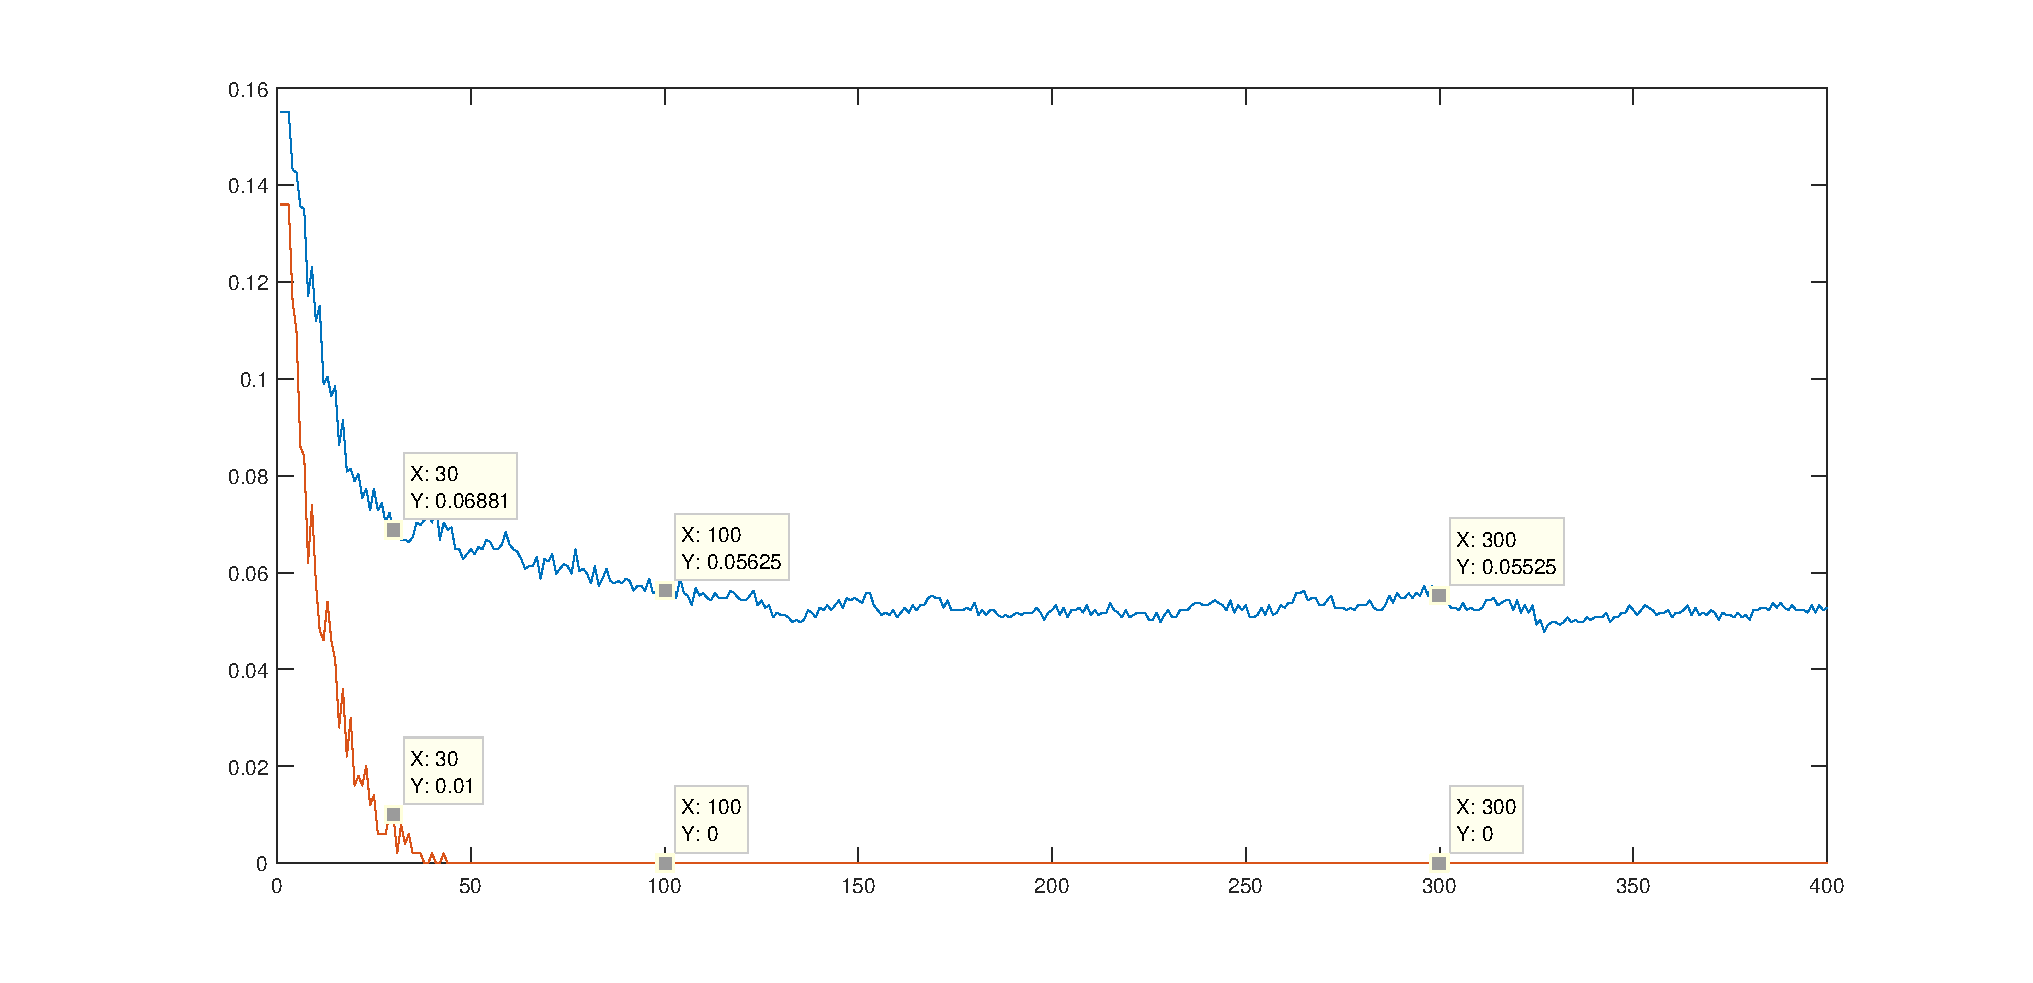
\includegraphics[width=\textwidth]{500trained.eps}
\caption{500个样本的训练错误率和测试错误率}
\label{fig1}
\end{figure}

\begin{figure}
\centering
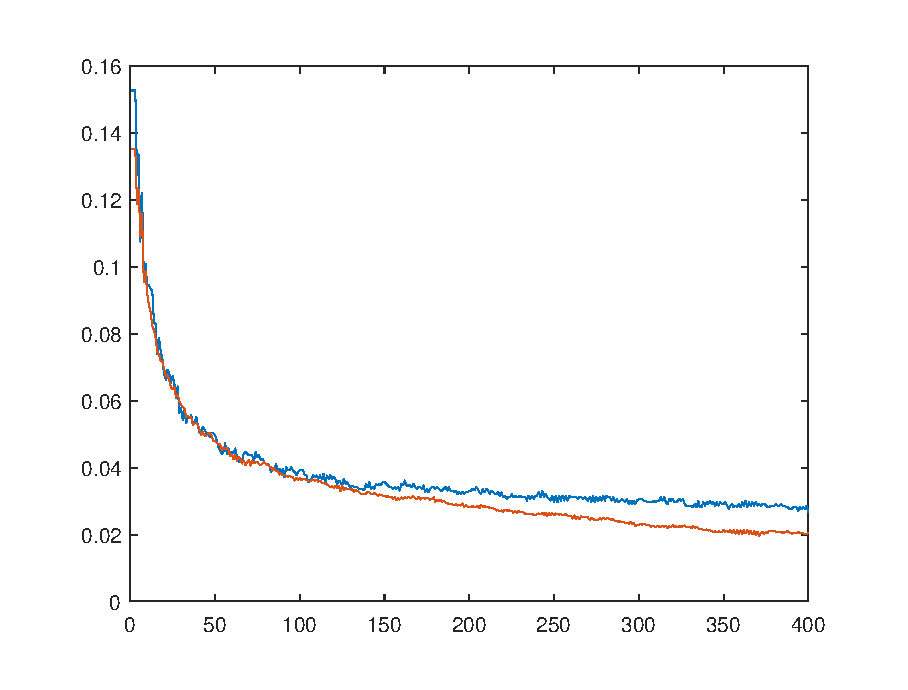
\includegraphics[width=\textwidth]{alltrained.eps}
\caption{所有训练集样本参与训练的训练错误率和测试错误率}
\label{fig2}
\end{figure}

具体的代码已经随附件一同提交,由于英文系统编码的问题,删去了注释的中文部分以提高可读性。

\subsection{决策树和随机森林的训练}
决策树和随机森林的训练错误率如图\ref{fig3}所示

\begin{figure}
\centering
\includegraphics[width=\textwidth]{Capture.JPG}
\caption{训练正确率(训练集自动分割20\%数据}
\label{fig3}
\end{figure}

在测试集上检查正确率可以得到
\begin{table}
\centering
\begin{tabular}{|c|c|c|}
\hline
训练类型&训练集上测试子集正确率&测试集上正确率\\
\hline
分裂数为4的决策树&90\%&88.95\%\\
\hline
分裂数为20的决策树&90\%&91.31\%\\
\hline
分裂数为100的决策树&90\%&91.31\%\\
\hline
30分类器随机森林&98\%&94.53\%\\
\hline
100分类器随机森林&96\%&96.23\%\\
\hline
300分类器随机森林&98\%&96.23\%\\
\hline
\end{tabular}
\end{table}
\subsection{总结}
从训练过程可以发现,不论是boosting方法还是bagging方法都可以在一定程度上提高决策树类型的正确率。决策树随着分裂数的增大,正确率能够得到一定程度上的提升,但是这个提升幅度很小而且会迅速趋向饱和。不论是bagging方法的的分类器数量和boosting方法的迭代数量的提升均可以提升正确率,但是也有一定的饱和上限,就本题而言,不论是bagging方法的分类器数量还是boosting方法的迭代次数到达100之后性能提升就很小了。

同时,bagging方法中出现98\%的高正确率可能是因为偶然因素导致的,之前几次的训练正确率在96\%左右。

\section{代码结构}
决策树和随机森林结构存贮在'tree\_wood.mat'中,400次迭代的Adaboost存储在'itera.mat'中

Adaboost程序入口在'stump-AdaBoost/main.m',决策树和随机森林程序入口在'main.m'中,测试在'test.m'中
\end{document}